\chapter{Logging}

Logging is quite a big problem in almost every system. At the moment in Seznam.cz we have a special library called dbglog which is used for logging from C/C++ and Python. This library is also open sourced \cite{dbglog}. You can configure it to log to stderr or to a file. It simply formats the message with data arguments add a general info, like file from which the log message has been called, the line number, the function name, the log level, current time and so on.

The text files take up a lot of space, so we had to think about storing information in a binary form or even compressed. Another idea was to store logs not as simple strings but in a structured form. That would be very helpful for a basic analysis of these debug logs, for example to check the number of records processed etc. We started to develop a complex logging solution quite a while ago. I implemented a library for storing data to binary files. The library is in Go and uses the Apache Kafka \cite{kafka} file format. Picking the Kafka file format was quite an easy decision, as we wanted to use the Kafka cluster as a logging service where all our applications will send their logs. Then we can decide which logs go to the Elasticsearch \cite{elasticsearch} for a human analysis and which will go to the HDFS \cite{hdfs} for permanent storage and time consuming calculations. And of course in the future more approaches can come. Kafka file format also supports compression and storing partition key in each message.

A very common problem with logging into file system is rotating files. There are many approaches for this, but logrotate or another similar daemon running in the background is not the way we want to go in Docker. The Docker principle is to have only one process in one container. Sure you can run logrotate in another container in pod and send signals from one container to the other, but that’s generally not a good idea. That’s why the library for storing logs into file system also supports file rotation.

So at the moment I have solved the problem with file rotation and storing files from our applications. But how to deal with logs from any third part application? Actually the answer is very easy as well. Does the application support logging to stderr? If so, just make use of it and throw a pipeline to send the stream to stdin for another application which will simply save each line into my library. If stderr is not an option (for example nginx), does the application support syslog interface? If so, do exactly the same, only that the application which reads it will have to expose the syslog interface.

So now I have the files stored at the file system. How to send them to Kafka for further processing? This simple task proved to be quite tricky. There are several daemons which read files and send them somewhere. Kubernetes also have one of them.

\section{FluentD}

Fluentd is an open source data collector for a unified logging layer. The Fluentd allows to unify data collection and consumption for a better use and understanding of data \cite{fluentd}.

\begin{figure}[htb]\centering
  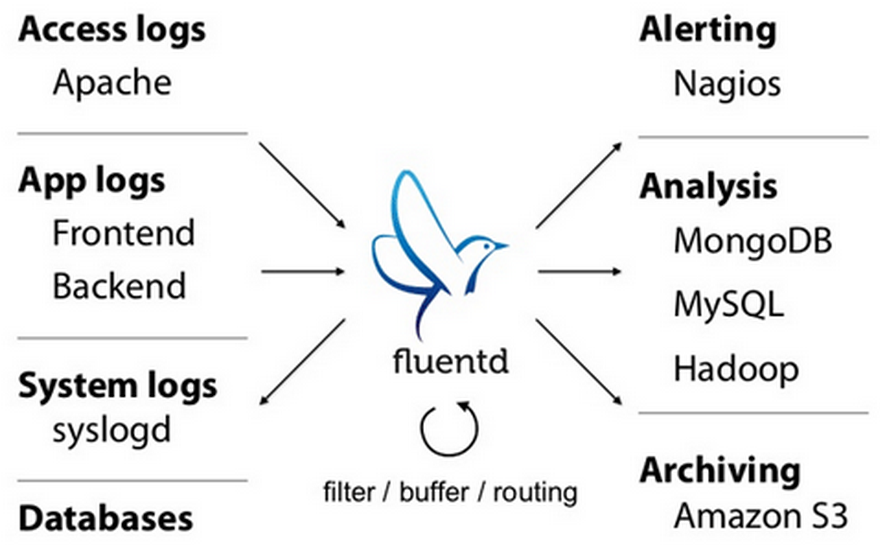
\includegraphics[width=1\textwidth]{images/fluentd-architecture.png}
  \caption
    [fluentd]
    {fluentd \cite{fluentd}}
  \label{fig:fluentd}
\end{figure}
 
The Fluentd is natively implemented in Kubernetes but there is a couple of problems. The first one is that plugins for The Fluentd are written in Ruby \cite{ruby}, which is not used in Seznam.cz, so writing a custom plugin could become an issue. And we already know we would need at least one custom input plugin for reading the Kafka file format. The second problem is that in the default configuration the Fluentd reads from the input file, stores those data in a memory buffer and tries to send them to Kafka. When the Fluentd, its pod or even the whole node fails, the data are lost and when it starts again it does not know about the power cut and it starts from the last known position in the file. This all means that the Fluentd is not an option for us.

\section{Logstash}
Logstash is a tool for managing events and logs. It can be used to collect logs, parse them, and store them for later use (e.g. for searching) \cite{logstash}.
 
Logstash plugins are written in JRuby so it’s almost the same as with Fluentd. We tried to use Logstash in the current conditions at Seznam.cz but it completely failed because of memory demands. Logstash is written in Ruby but runs under JVM, so its memory demands are huge. We also wanted to have one log forwarder from the file system to the Kafka for each pod so that the failure of one pod won’t affect other pods and with Logstash’s memory usage this is not possible.
    
\section{Heka}
Heka \cite{heka} is written in Go, its plugins are written in Go and that is an advantage over Logstash or Fluentd. Heka also supports sandboxed Lua for filter scripting without the need to recompile Heka. There are plugins for Apache Kafka, Elasticsearch and many other outputs. That’s why I started to examine Heka more closely.

Heka is a heavily plugin based system. There are six different types of Heka plugins \cite{heka}:
\begin{itemize}
  \item	Inputs
    \begin{itemize}
      \item Input plugins acquire data from the outside world and inject it into the Heka pipeline. They can do this by reading files from a file system, actively making network connections to acquire data from remote servers, listening on a network socket for external actors to push data in, launching processes on the local system to gather arbitrary data, or any other mechanism.
    \end{itemize}
  \item	Splitters
    \begin{itemize}
      \item Splitter plugins receive the data that is being acquired by an input plugin and slice it up into individual records.
    \end{itemize}
  \item	Decoders
    \begin{itemize}
      \item Decoder plugins convert data that comes in through the Input plugins to Heka’s internal Message data structure. Typically decoders are responsible for any parsing, deserializing, or extracting of structure from unstructured data that needs to happen.
    \end{itemize}    
  \item Filters
    \begin{itemize}
      \item Filter plugins are Heka’s processing engines. They are configured to receive messages matching certain specific characteristics (using Heka’s Message Matcher Syntax) and are able to perform arbitrary monitoring, aggregation, and/or processing of the data. Filters are also able to generate new messages that can be reinjected into the Heka pipeline, such as summary messages containing aggregate data, notification messages in cases where suspicious anomalies are detected, or circular buffer data messages that will show up as real time graphs in Heka’s dashboard. 
    \end{itemize}
  \item	Encoders
    \begin{itemize}
      \item Encoder plugins are the inverse of Decoders. They generate arbitrary byte streams using data extracted from Heka Message structs. Encoders are embedded within Output plugins; Encoders handle the serialization, Outputs handle the details of interacting with the outside world.
    \end{itemize}
  \item	Outputs
    \begin{itemize}
      \item Output plugins send data that has been serialized by an Encoder to some external destination. They handle all of the details of interacting with the network, filesystem, or any other outside resource. They are, like Filters, configured using Heka’s Message Matcher Syntax so they will only receive and deliver messages matching certain characteristics.
    \end{itemize}
\end{itemize}

I developed a custom splitter plugin and a custom decoder in Go, which are able to split and decode data from the Kafka file format. So the default Heka plugin -- Logstream Input -- reads bytes from the Kafka files, the Kafkalog splitter and the Kafkalog decoder create Heka messages which are send through the filters to a simple encoder and to the Kafka output.

When Kafka ran, everything seemed fine and worked as expected. The problems started when I stressed Kafka. I shutdown some of the brokers and watched how Heka can handle it. Heka noticed that one or more Kafka brokers were down and the rest was in the middle of the leader election, but it didn’t stop trying to send messages. It slowed down, because of the timeouts that occurred, but after a while the message that cannot be delivered to Kafka is dropped down and the Input plugin reads new bytes from the file. I tried to simulate Heka failure, simply by Linux kill command.

The Logstream input plugin keeps a journal file. In the journal there is the file name, the offset of the last read message and the control hash. But the problem is, that input plugins do not cooperate with outputs. Heka is highly expandable with plugins. One input can generate message to Heka’s pipeline and more outputs can read them and do something with them. Filters can drop messages or create new messages so there is no simple way to synchronize the input and the output plugin. Which means there is a risk of losing messages.
 
I did a research about Heka’s reliability and found a couple of some e-mails and discussions where the Heka authors are saying that 100 \% reliability was never their goal. But we need it at Seznam.cz as we can’t say that some logs will possibly be lost. So I try to fix this.

The Kafka output plugin uses the Sarama library from Shopify \cite{shopify} to communicate with Kafka. There is a synchronous and an asynchronous Kafka producer. In the output plugin the asynchronous one is used. The asynchronous producer is faster, because it does not wait for errors or success confirmation. All messages are handled in separate goroutines\footnote{A goroutine is a lightweight thread managed by the Go runtime \cite{goroutine}.}. Producer errors are handled in output plugin, but only to be logged and dropped down. I fixed this with a special error channel addition. When an error occurs, it is sent to the error channel and the main goroutine which process Heka messages starts fixing it. When there is an error I don’t want to process any other messages from the Heka pipeline, the backpressure is desirable. I create one extra synchronous Kafka producer with exactly the same configuration as the main (async) one and the error is sent through it. The maximum number of attempts is configurable and can even be set to infinity. Dealing with the error through the synchronous producer will not read from the main message channel, which can fill up eventually. This causes a backpressure and Heka will stop in such case (of course, only under the condition that no other output processes the input messages).

I have tested this by writing a Kafka consumer in Python and uploading files with a few millions of numbered messages. The consumer reads everything from the special topic and looks for holes and duplicates in sorted sequence of messages. I randomly shut down Kafka brokers, even whole Kafka, simulating packet lost with Linux iptables DROP directives and watched consumer’s statistics. It turned out that with a few millions of messages there is a few thousands of duplicates but no miss. Duplicates can also be caused by consumer, because Kafka’s philosophy is to deliver each message at least once. And duplicates are no problem for us, because we can easily discover them. This fix seems quite useful and generic, so I will try to send it to the upstream as a merge request.

Fixing this issue will only try to repeat errors when they occurs. This does not solve the next problem, when Heka input plugin reads something from a file, it confirms the new offset to its journal file and sends the message to the Heka pipeline. If Heka fails now, the memory buffer will be lost and after a new start the input file will seek to the position from the journal file. I need to figure out how to fix this too. 

The problem is, that one input can be processed by more outputs, and also more inputs can be processed by a single output. The input and the output plugins don’t know about each other. I think there is not one generic solution for this problem. The best what I could come out with is the following idea:

\begin{itemize}
  \item Each input plugin will be working as is plus it will be adding filename, offset and its name as fields to the message. 
  \item The output plugin will be also working as is plus it will read the success message from Kafka, confirming that message was delivered to it. Output saves those metadata sent from input to its private variable and once in a while it sends a special message: an acknowledgement consisting from the filename, the offset and the name of the input plugin.
  \item I will write a new plugin, the Checkpointer, which will consume acknowledgements from the output and save checkpoint files per each input. This plugin has to know which outputs consume messages from which inputs to be able to successfully maintain acknowledgements from more output that consumes from single input.
\end{itemize}

This theoretical idea might be good, but it is unfeasible in practice. The main problem is, that output plugins are not allowed to generate new messages. Also the condition to know about all other plugins is senseless in Heka.

So I have to update my idea to be implementable in Heka and useful for Seznam.cz. Our applications logs through my library, which rotates file and is using our naming convention: \lstinline{datetime-timezone-rotate_interval-component_name-postfix.szn}. One application can generate more files with different postfix value. For example \lstinline{szn-fulltext-NAME-dbg} and \lstinline{szn-fulltext-NAME-event}. In the log directory, there is a \lstinline{kafkafeeder.yaml} file -- with our generic configuration where to send files, how long to retain them and so on. That means in our conditions it is possible to always have one input for one output. The problem that output plugins are not able to send new messages can be solved by implementing the checkpointer logic right into the Kafka output, so it will be saving checkpoint files to the file system.

There have to be written a new binary, which will start, copy checkpoints to journals, transform Kafkafeeder configuration to a Heka specific configuration format, start Heka with some predefined options, watch checkpoints and data in a separate goroutine and delete old (and successfully uploaded) log files from filesystem.

This solution will be 100 \% reliable but it is also Seznam.cz specific, because our custom binary (let’s call it Kafkafeeder) will transform our custom configuration to the Heka format  and it will create one Input plugin for one Output plugin with a unique name, so checkpoints can be saved and reused as journal files of those Inputs.
 
\subsection{Kafkafeeder}
I started designing this application in Go. The Kafkafeeder has to:
\begin{itemize} 
  \item	Copy checkpoints to journal directory
  \item	Start Heka daemon (\lstinline{hekad})
  \item	Monitor log directory for changes
    \begin{itemize}
      \item Reload when it finds a new \lstinline{kafkafeeder.yaml} or when an existing one disappears
    \end{itemize}
  \item	Convert the \lstinline{kafkafeeder.yaml} custom configuration to the Heka format and reload hekad 
  \item	Monitor checkpoints and delete old and successfully uploaded logs from the directory
\end{itemize}

The application is made as a five goroutine architecture, where the main goroutine initializes all the necessary objects and starts all other goroutines.

The cleaner goroutine is responsible for removing old logs, which have been successfully sent to Kafka. Successful dispatch may be tracked from checkpoint files generated by heka. All files with their last modification time older than the retention duration in the configuration file will be deleted.

The signal goroutine is waiting for system signals and handles them properly. When \lstinline{SIGTERM} is captured, the main shutdown function is called and the whole application stops safely. When \lstinline{SIGCHLD} signal is captured forked child is dead and so I have to check if it should be running. If so, a problem occurred and the main shutdown function is called.

The watcher goroutine periodically watches the directory with logs. When \lstinline{kafkafeeder.yaml} file is found it is registered to LogManager object. After all new logs are registered, the keepValid function is called so the LogManager will keep only those records that actually exists. If something was changed, the reload is called.

The hekad goroutine is responsible for copying checkpoint files to the Heka journal files and starting, stopping and checking hekadCmd. Also when the reload is called, the hekad goroutine converts all logs from LogManger to the Heka specific configuration.

HekadCmd is a wrapper around the actual hekad process. This wrapper sends signals to forked process, captures its standard output and error and logs all messages via the internal logger.

\begin{figure}[htb]\centering
  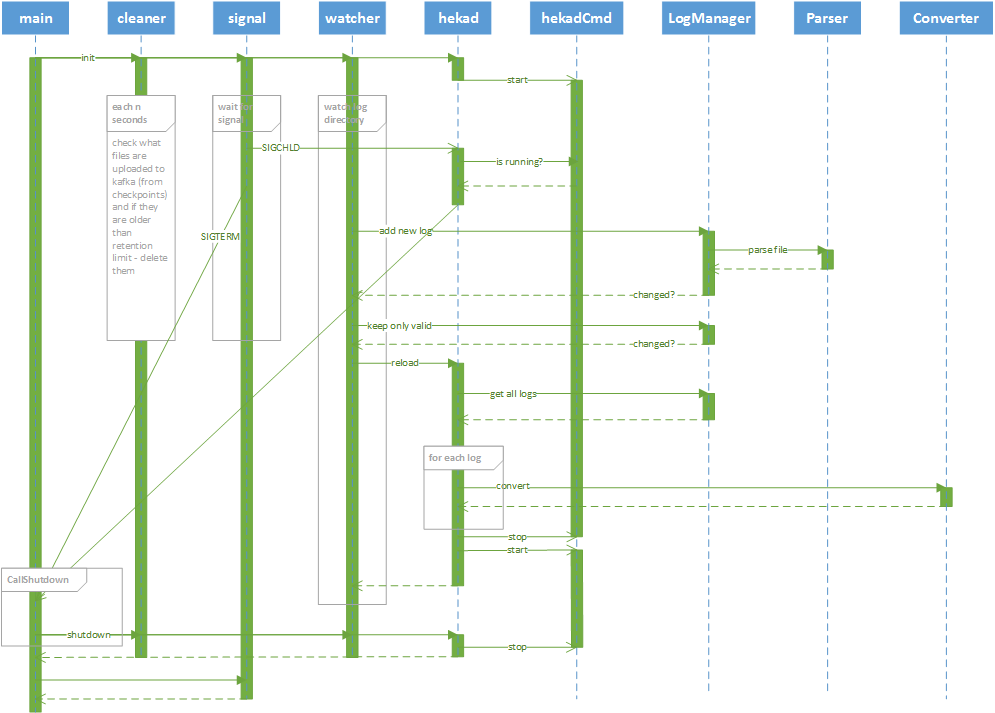
\includegraphics[width=1\textwidth]{images/kafkafeeder.png}
  \caption
    [Kafkafeeder architecture]
    {Kafkafeeder architecture}
  \label{fig:kafkafeeder}
\end{figure}
                            
